\documentclass[11pt]{article}

\usepackage{silence}
\WarningFilter{biblatex}{Patching footnotes failed}
\usepackage[
style=authoryear,
natbib
]{biblatex}
\addbibresource{bibliography.bib}

\usepackage{graphicx}
\usepackage{caption} % More complex captioning
\usepackage{subcaption} % subfigure environment and co.
\usepackage{placeins} % \FloatBarrier flushes the float buffer

\usepackage{amsmath}
\usepackage{amssymb}
\usepackage{bbold}

\usepackage{tikz}
\usetikzlibrary{positioning}
\usepackage[linguistics]{forest}
\usetikzlibrary{tikzmark}

\usepackage[normalem]{ulem} % \sout strikethrough text

\usepackage{gb4e}

\newcommand{\ok}{\checkmark}
\DeclareMathOperator{\bbexists}{\exists\mskip-7mu\exists}


\title{Senior Thesis Proposal}
\author{Benjamin Kyle Olson}
\date{2026-11-07}

\begin{document}
\maketitle

\section{Introduction}

This thesis is to explain relative clauses out of expletive \textit{there} contexts (TRCs) such as (\ref{ex:trc}). These are known to exhibit determiner selection (\ref{ex:det}): broadly, definites and universals are acceptable; indefinites are unacceptable. This is particularly striking against the well-known (anti)definiteness effect (DE) of expletive \textit{there} contexts (TCs) seen in (\ref{ex:def}).

\begin{exe}
	\ex {The cat that there was in the room jumped out the window.}\label{ex:trc}\footnote{\label{fn:intro}TRCs seem to be almost universally partially marked and informants consistently say that they would prefer the plain relative clauses without expletive \textit{there}. I think this partially has to do with the generally presentationality of TCs (e.g. \cite{zucchiIngredientsDefinitenessDefiniteness1995}). Part of the research phase of this project will include trying to find less marked examples, ideally even contexts where the TRC is required/better than the plain relative. One such variable seems to be tense: informants sometimes report varying acceptability depending on past vs. present tense; puzzling this seems to be ideolectical and unstable in the sense that the other tense is more available once you ``figure it out.''}
	\ex {\textbf{Determiner Selection:} (\cite{carlsonAmountRelatives1977}, ex. 10a, 10e, 11b)
		\begin{xlist}
			\ex[]  {The people there were at that time only lived a few decades.}
			\ex[]  {Every lion there is eats meat.}
			\ex[*] {A man there was disagreed.}
		\end{xlist}}\label{ex:det}
	\ex {\textbf{Definiteness Effect:} (\cite{milsarkExistentialSentencesEnglish1974}, ch. 1, ex. 12a-b)
		\begin{xlist}
			\ex[]  {There will be a duck roasted on Arbor Day.}
			\ex[*] {There will be the duck roasted on Arbor Day.}
		\end{xlist}}\label{ex:def}
\end{exe}

These determiners seem to be just those that regularly allow dynamic reference. The marked continuations in (\ref{ex:dynamic-determiners}) seem distinctly odd, especially compared to their unmarked siblings.\footnote{Of course, the judgements here are noticably less sharp than the TRCs above; I have three resolutions to this snag: (i) It seems entirely reasonable to believe that determiner reference is, in a sense, looser with distinct sentences than with relative clauses. (ii) The determiner restrictions do not seem iron-clad: as \citet{grosuAmountRelatives2017} point out, certain indefinites sometimes permit some kind of partitive interpretation:
	\begin{exe}
		\ex {Some students that there were at the party left early, but the remainder stayed past midnight. \\ (\citet{grosuAmountRelatives2017} ex. 25a)}
	\end{exe}
	(iii) Finally, given the general weakness of TRC determiner restrictions, it would be good to run an acceptability experiment to see how strong these patterns really are.}

\begin{exe}
	\ex {\begin{xlist}
			\ex {There is a cat in the hat.
				\begin{xlist}
					\ex[] {The cat jumps out the window.}
					\ex[??] {A cat jumps out the window.}
				\end{xlist}}
			\ex {There are three cats in the hat.
				\begin{xlist}
					\ex[] {The three cats jump out the window.}
					\ex[] {Every cat jumps out the window.}
					\ex[??] {Three cats jumps out the window.}
					\ex[??] {Most cats jumps out the window.}
				\end{xlist}}
		\end{xlist}}\label{ex:dynamic-determiners}
\end{exe}

\begin{figure}[htbp]
	\centering
	\begin{subfigure}{.42\textwidth}
		\begin{center}
			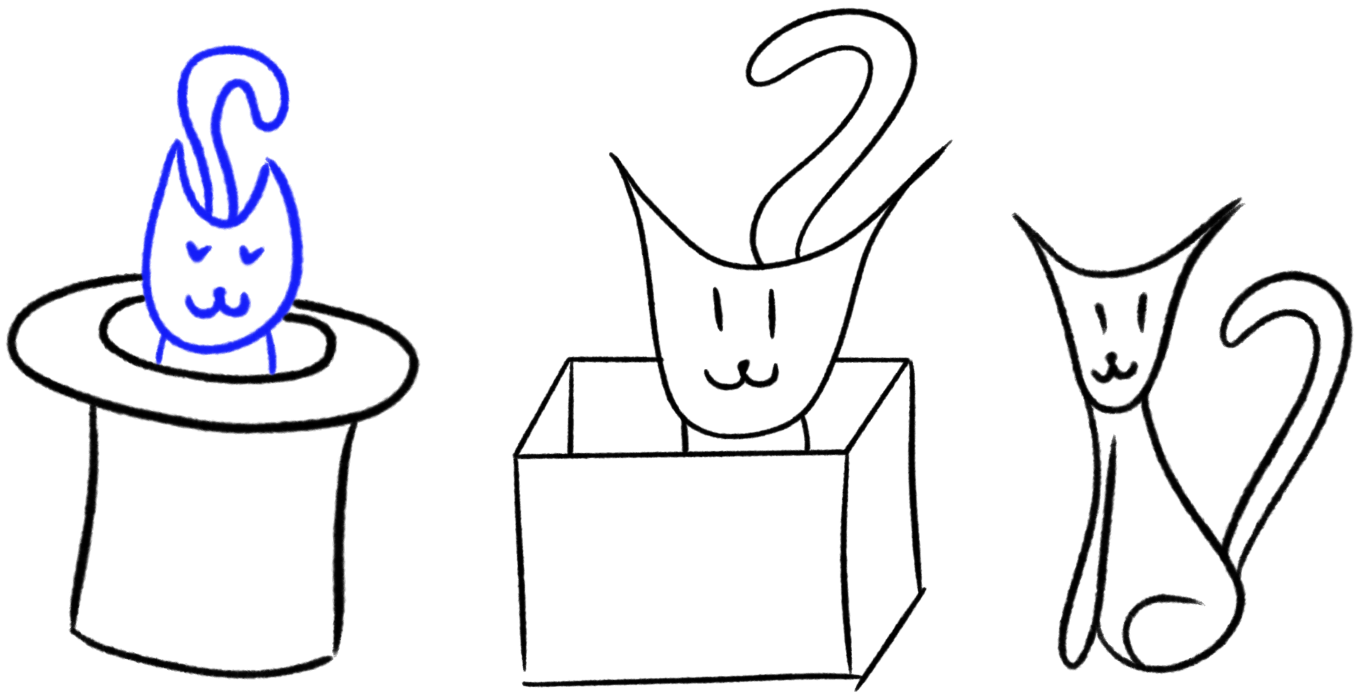
\includegraphics[width=0.95\textwidth]{figures/absolute.png}
			\captionsetup{justification=centering,format=hang}
			\caption{Absolute context, \\ exactly one hat}\label{fig:absolute}
		\end{center}
	\end{subfigure}\ %
	%
	\begin{subfigure}{.57\textwidth}
		\begin{center}
			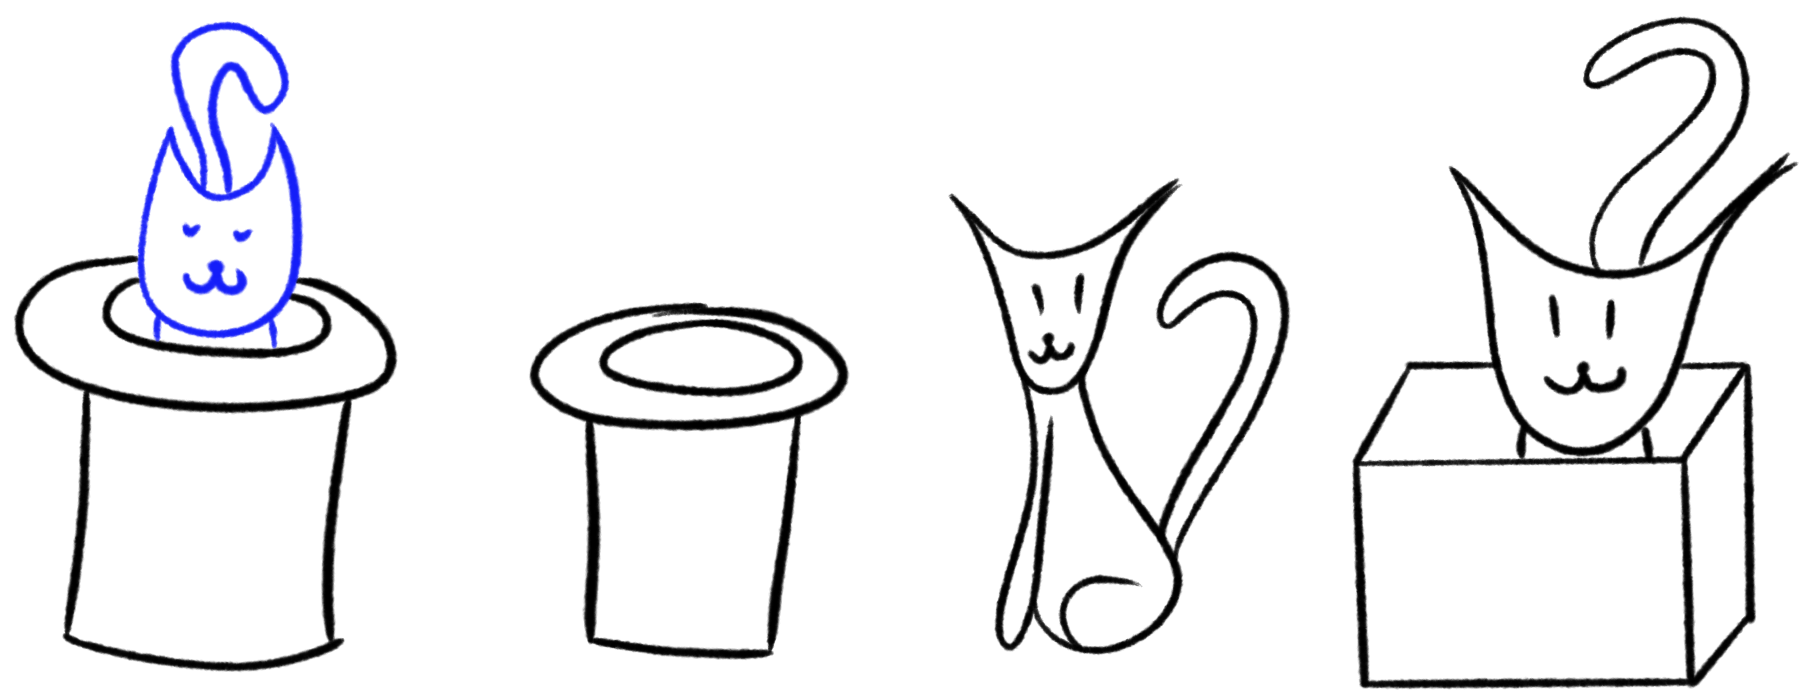
\includegraphics[width=0.95\textwidth]{figures/haddock.png}
			\caption{Haddock context, \\ several hats}\label{fig:haddock}
		\end{center}
	\end{subfigure}

	\begin{subfigure}{.25\textwidth}
		\begin{center}
			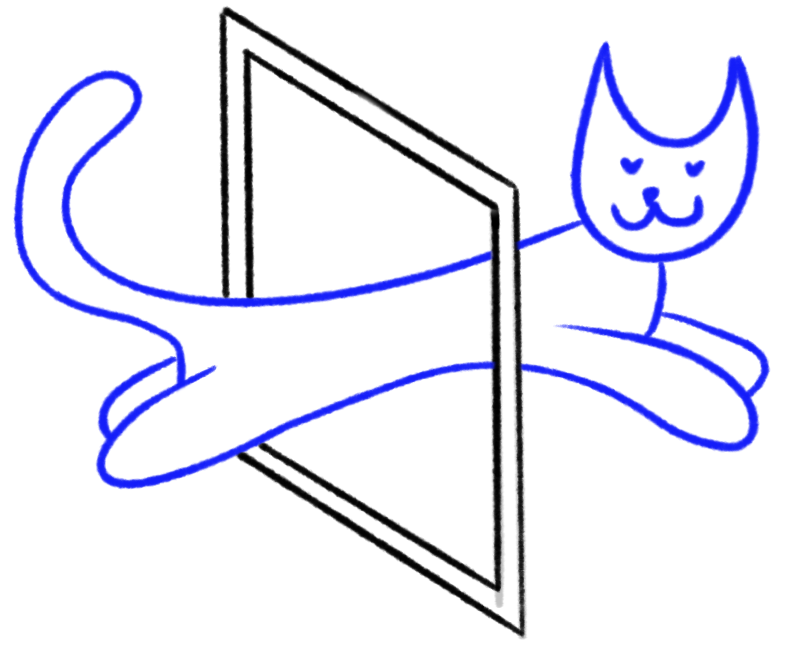
\includegraphics[width=.95\textwidth]{figures/window-jumping.png}
		\end{center}
		\caption{Window jumping}
	\end{subfigure}
	\caption{(\ref{ex:haddock}) Contexts}
\end{figure}

Finally, I have novel data concerning superlative Haddock readings with regards to TRCs: First, consider a classic Haddock context of multiple hats and multiple cats, but only one hat with any cats and only one cat in any hats as in Figure~\ref{fig:haddock}; if indeed that one hatted-cat jumped out the window, (\ref{ex:haddock}) shows that TRCs may felicitously take Haddock readings.\footnote{\ok marks indicate available readings, * marks indicate unavailable readings.}

\begin{exe}
	\ex {\textbf{Haddock TRC:} \\
		The cat that there is in the hat jumps out the window.
		\begin{xlist}
			\ex {(\ok Absolute; Fig.~\ref{fig:absolute}) There is a cat in the (unique) hat. The cat jumps out the window.}
			\ex {(\ok Haddock; Fig.~\ref{fig:haddock}) There is a cat in a hat. The cat jumps out the window.\footnote{Note that a cat in the second hat would make this reading infelicitous as such would fail to satisfy uniqueness for the head determiner (i.e. item 1 in ex. \ref{ex:haddock}). This is predicted by the definite determiner at the start of the second sentence in the paraphrase (\ref{ex:haddock-sem})}}\label{ex:haddock-sem}
		\end{xlist}}\label{ex:haddock}
\end{exe}

\begin{figure}[htbp]
	\centering
	\begin{subfigure}{.5\textwidth}
		\begin{center}
			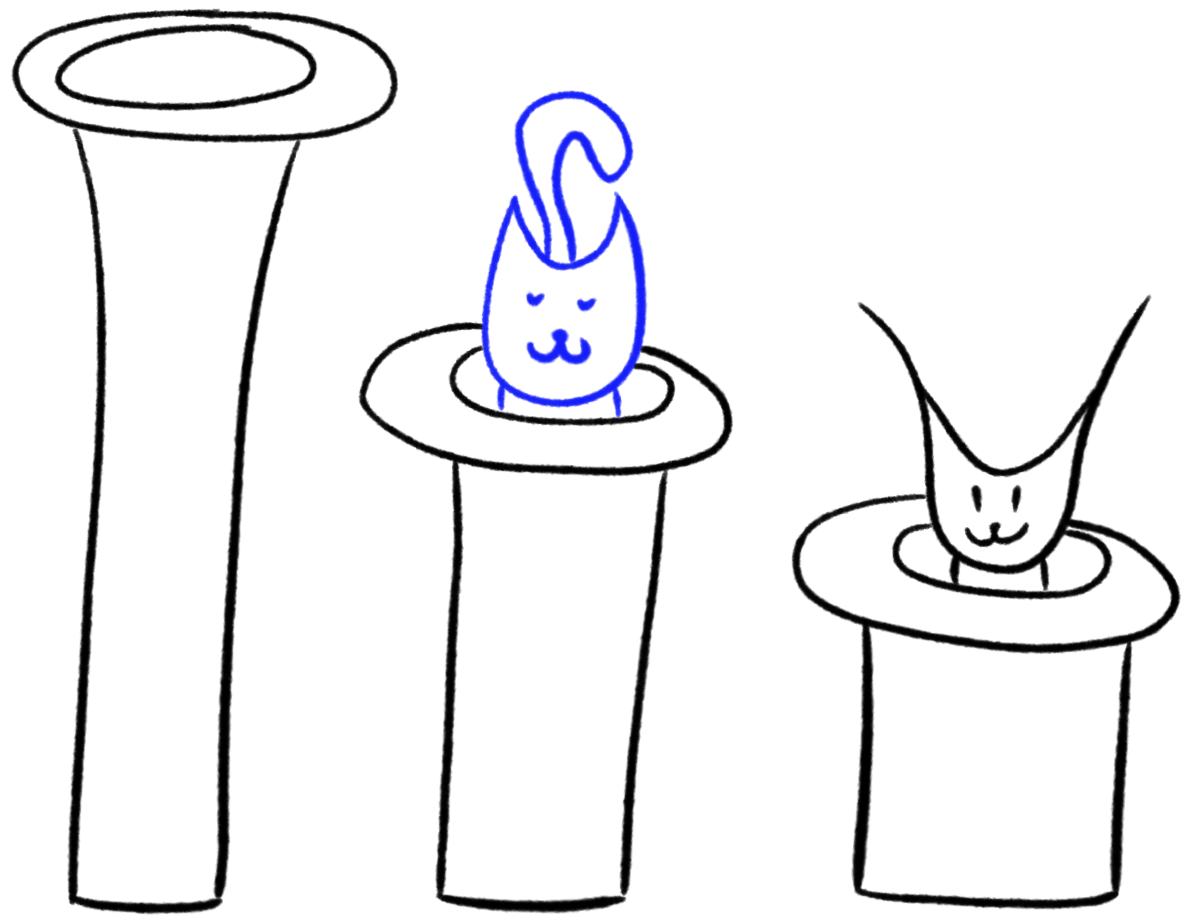
\includegraphics[width=0.95\textwidth]{figures/superlative-haddock.png}
		\end{center}
		\caption{Superlative Haddock context}\label{fig:superlative-haddock}
	\end{subfigure}%
	%
	\begin{subfigure}{.25\textwidth}
		\begin{center}
			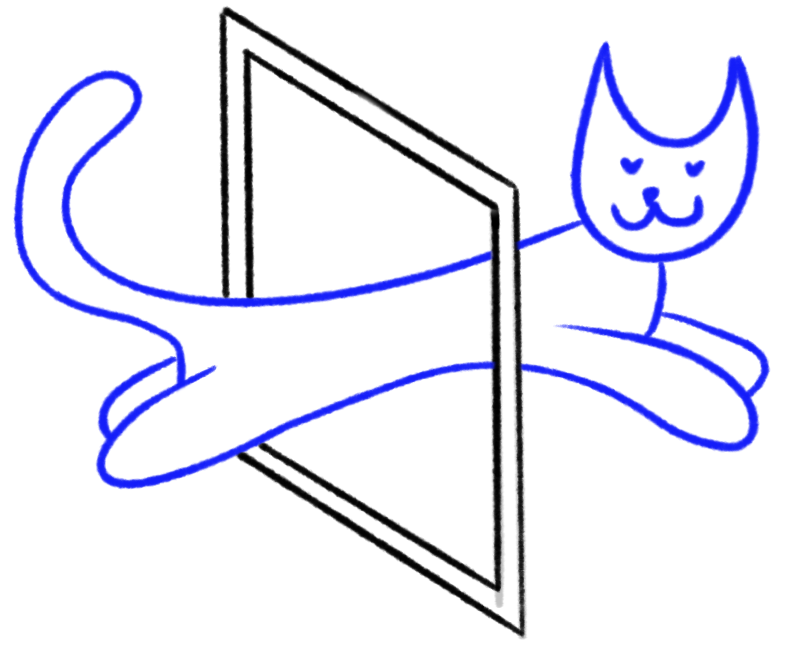
\includegraphics[width=.95\textwidth]{figures/window-jumping.png}
		\end{center}
		\caption{Window jumping}
	\end{subfigure}
	\caption{Superlative Haddock (\ref{ex:sup-haddock}, \ref{ex:trc-sup-haddock}) context}
\end{figure}

Now, we expand our context with hats of various tall-ness and permit many cats across the hats, so long as there is only one tallest of the hats bearing any cats, and one cat in said hat as in Figure~\ref{fig:superlative-haddock} (and indeed that that cat jumped out the window), then we see (\ref{ex:sup-haddock}) may take a (relative) superlative Haddock reading.

\begin{exe}
	\ex {\textbf{(Relative) Superlative Haddock:} \\
		The cat that is in the tallest hat jumps out the window.
		\begin{xlist}
			\ex {(\ok Absolute) There is a cat in the (absolutely) tallest hat. The cat jumps out the window.\footnote{Note that Fig.~\ref{fig:superlative-haddock} is infelicitous with an absolute reading like (\ref{ex:abs-sup-sem}) since the context does not, in fact, have a cat in the absolutely tallest hat.}}\label{ex:abs-sup-sem}
			\ex {(\ok Haddock; Fig.~\ref{fig:superlative-haddock}) There is a cat in the (relatively) tallest hat with any cats in it. The cat jumps out the window.\footnote{Note that removing the cat from the shortest hat substantially worsens (\ref{ex:sup-haddock}), presumably for something like \citet{schlenkerMinimizeRestrictorsNotes2005}'s \textit{Minimize Restrictors}: it is pragmatically odd to impose a superlative on a singleton.}}
		\end{xlist}}\label{ex:sup-haddock}
\end{exe}

However, we see that the analogous TRC (\ref{ex:trc-sup-haddock}) is infelicitous, permitting only an absolute reading in which there is a universally tallest hat.

\begin{exe}
	\ex {\textbf{TRCed Superlative Haddock:} \\
		The cat that there is in the tallest hat jumps out the window.\\
		(\ok Absolute, * Haddock)}\label{ex:trc-sup-haddock}
\end{exe}

\subsection{Complications}
The landscape is further muddied by the fact that apparently TRCs \textit{may} take superlative Haddocks in certain situations such as the modal context of (\ref{ex:de-dicto-sup-haddock}): the sentence seems fine even if it is guarenteed that there is an absolutely tallest hat and that hat never has a cat in it.

\begin{exe}
	\ex {\textbf{\textit{De dicto} TRCed Superlative Haddock:} \\
		I will adopt the cat that there is in the tallest hat.
		\begin{xlist}
			\ex {(\textit{de re}) There is a cat in the tallest hat. I will adopt the cat. \\
				(\ok Absolute, * Haddock; exactly as in ex. \ref{ex:trc-sup-haddock}).}
			\ex {(\textit{de dicto}) There will be cats in hats of various tallness. In particular, there will be a cat the tallest hat. I will adopt the cat. (\ok Absolute, \ok Haddock.)}
		\end{xlist}}\label{ex:de-dicto-sup-haddock}
\end{exe}

This seems to be a product of intensions: given the context (\ref{ex:context:modal}), I can felititously make the generalization (\ref{ex:modal}). Curiously, (\ref{ex:modal}) seems less acceptable if, throughout the video, the autodefenestrating cat was never in the absolutely tallest hat.

\begin{exe}
	\ex {\textbf{Modal TRCed Superlative Haddock:}\footnote{Adapted from a suggestion by Leon Cosgrove, p.c.}
		\begin{xlist}
			\ex {\textit{Context: A cruel veterinarian has, over the course of her 20-year career, engaged in the habit of placing infirm cats into a bunch of hats of varying heights. She has 5 hats, each of different height, but puts at most only 3 cats at any one time in one each. Those hats are evilly positioned adjacent to a window. Without fail, that cat positioned in the one hat tallest w.r.t. the other two would leap out of the hat and out the window. She has evilly recorded these events of cat autodefenestration, editted them together as a montage, and showed me this video.}}\label{ex:context:modal}
			\ex {The cat that there was in the tallest hat would jump out the window. (\ok Absolute, \ok Haddock)}\label{ex:modal}
		\end{xlist}}\label{ex:modal-trc}
\end{exe}

I will note that the difference between any acceptability does not seem to be a subject-object distinction: allodefenestration from Haddock tallest hats in (\ref{ex:allodefenestration}) is as unacceptable as autodefenestration in (\ref{ex:trc-sup-haddock}).

\begin{exe}
	\ex {John threw the cat that there was in the tallest hat out the window. \\
		(\ok Absolute, * Haddock)}\label{ex:allodefenestration}
\end{exe}

\subsubsection{Interim Summary}
To recapitulate the data just above: definites and universals determiners, but not indefinites, may generally co-occur with TRCs (\ref{ex:det}). These seem to be those determiners which regularly permit dynamic reference (\ref{ex:dynamic-determiners}). Separately, TRCs may take plain Haddock readings (\ref{ex:haddock}) but generally not superlative Haddocks (\ref{ex:sup-haddock}). Finally, TRCed superlative Haddocks \textit{are} available in modalized/possible-worlds contexts (\ref{ex:de-dicto-sup-haddock}-\ref{ex:modal-trc}).

\subsection{Hypothesis}
The present hypothesis proposes that both these effects---those determiner restrictions and superlative Haddocks---may be resolved by appealing to dynamic semantics. The head determiner selection is seen as just those determiners which regularly permit dynamic reference.

Meanwhile, the determiner associated with the superlative---`the (tallest hat)'---is split into a definite uniqueness check \(\mathbb{1}\) and indefinite introduction \(\bbexists\) following \citet{bumfordSplitscopeEffectsDefinite2017}. In this way, Haddock readings are garnered by scoping/interleaving the definiteness of hats \(\mathbb{1}_h\) over the indefiniteness of cats \(\bbexists_c\): \(\mathbb{1}_c > \mathbb{1}_h > \bbexists_h > \bbexists_h\); absolute readings flip the central relation: \(\mathbb{1}_c > \bbexists_c > \mathbb{1}_h > \bbexists_h\).
Importantly, the scope of \(\mathbb{1}\) may be trapped within the TRC, presumably by \textit{there}, such as when including superlative force. The desired results of the data should be achievable then by further considering a dynamic semantics. One potential syntactic configuration is given in Figure~\ref{fig:tree-rel-sup}.

\begin{figure}
	\makebox[\textwidth][c]{
		\begin{forest}
			[DP [D [the [\(\mathbb{1}_c\) ]]]
			[NP [NP [cat,roof ]]
			[CP [C [that ]]
			[IP [DP [there [there,name=there] [\(\mathbb{1}_h\),name=spec IP [\(\mathbb{1}_h\) ] [tallest_h,name=tallest ]]]]
			[I^\prime{} [I [{[+ pres]} ]]
			[VP,name=VP
			[VP [V [be ]]
				[DP [D [\(\bbexists_c\) ]] [NP [cat,roof ]]]]
			[{XP = PP} [P [in ]]
				[DP [D [the [\sout{\(\mathbb{1}_h\)},name=low def [\(\mathbb{1}_h\) ] [tallest_h,name=low def sup ]]
										[\(\bbexists_h\) ]]]
						[NP [AdjP [\sout{tallest_h},name=low sup ]]
								[NP [hat,roof ]]]]]]]]]]]
			% \draw[->] (spec VP) to[out=west, in=south] (spec IP);
			\draw[->] (low sup) to[out=south,in=east] (low def sup);
			\node[below=of spec IP] (a) {};
			\draw[->] (low def) to[out=west, in=south, looseness=1.5] (a);
			\draw[->, color=red, thick] (there) to node[pos=0.65,rotate=45] {\(\boldsymbol{\times}\)} (tallest);
		\end{forest}}
	\caption{The cat that there is in the tallest hat\dots{} (\ref{ex:haddock})}\label{fig:tree-rel-sup}
\end{figure}

\subsection{On Carlson's Restrictions}
I would be remise to ignore some puzzles from the literature: depending on individual judgements (\cite{heimWhereDoesDefiniteness1987}), TRCs seem to pattern with true amount relatives (i.e. of \cite{mendiaAmountRelativesRedux2017}) with respect to relativizer restrictions (\(\varnothing\), \textit{that}, never \textit{wh}-forms) and stacking facts (at most one amount relative/TRC). I ignore both of these as (i) they are particularly weak if ever applicable for my own dialect and (ii) I have independent reasons to believe they are more complex that given at face value: First, \citet{kayThatVsWhich} suggests that true amount relatives do not have this relativizer restriction. Second, to my knowledge, past research has not considered mixed stacking as in (\ref{ex:mixed}), particularly of amount, restrictive, and \textit{there} relative clauses in their many permutations. Third, in complex Haddock contexts like (\ref{ex:split})---such that there were several cats in the room and (later) in the kitchen, but only one (ever) in both (which of course jumped out the window)---stacking TRCs seems to be acceptable.

\begin{exe}
	\ex {It would take all day to feed the (number of) cats that there were on the island that the vet put down last year.}\label{ex:mixed}
	\ex {The cat that there was in the hat that that there was later in the kitchen jumped out the window.}\label{ex:split}
\end{exe}

\subsection{Further Mysteries}

Finally, I wish note some further phenomenon of which I may take up, but are not central to the project. For that reason, I will simply state them without further comment. First amongst these are (external) verbal TRCs as in (\ref{ex:verbal-trc}), which informants consistently report as entirely unacceptable. Across the board movement in (\ref{ex:acd}) is acceptable. Also observe in (\ref{ex:cop-reduction}) that copula reduction is exceptionally unacceptable. Finally, TRCs seem to interact with the diagnostics of \citet{postalContrastingExtractionTypes1994} in odd ways, I invite the interested reader to said article and to construct examples as they go.

\begin{exe}
	\ex[*] {The the fierce tomcat that there walked into the room fought my dog.}\label{ex:verbal-trc}
	\ex {The bathroom that either there isn't \_\_ or is \_\_ in a weird place needs better signage.}\label{ex:acd}
	\ex {\begin{xlist}
			\ex[] {There's a cat in a hat.}
			\ex[] {The cat that's in a hat jumped out the window.}
			\ex[*] {The cat (that) there's in a hat jumped out the window.}
		\end{xlist}}\label{ex:cop-reduction}
\end{exe}

\section{Alternate Approaches}

\subsection{Amount Relatives}

TRCs have historically been analyzed as parallel to (true) amount relative clauses (ARCs) like (\ref{ex:arc}) (see \cite{carlsonAmountRelatives1977}; \cite{heimWhereDoesDefiniteness1987}; \cite{grosuStrangeRelativesThird1998}, \citeyear{grosuAmountRelatives2017}). Certainly, TRCs \textit{may} have amount readings as in (\ref{ex:a-trc}), which I call an A-TRC. It is important to not that these are \textit{not} the subject of the project. Where relevant entity-denoting TRCs may be called E-TRCs, though usually just TRCs.

\begin{exe}
	\ex {\textbf{Amount Relative Clause:} (\cite{heimWhereDoesDefiniteness1987}, ex. 40)\\
		It will take us the rest of our lives to drink the champagne that they spilled that evening.}\label{ex:arc}
	\ex {(Lisa Selkirk, p.c. to Irene Heim; so cited in \citet{vonfintelAmountRelativesMeaning1999}, original unknown) \\
		There isn't the water in the sink that there is in the bathtub.}\label{ex:a-trc}
\end{exe}

The short (and possibly oversimplified) version largely developed by \citeauthor{grosuStrangeRelativesThird1998} (\citeyear{grosuStrangeRelativesThird1998}, \citeyear{grosuAmountRelatives2017}) (GL) is that the DE prohibits individual abstraction (Carlson/Heim; though see \cite{postalContrastingExtractionTypes1994}) but permits abstraction of individual-degree pairs.\footnote{Taking the relativizer restrictions as real, Heim suggests a degree vs. individual split of the relativizers. Of course, this is irrelevant should the phenomenon not hold; and, in fact, \citet{kayThatVsWhich}'s data suggests degree abstraction and ARCs do not care about the choice of relativizer.} Motivated partially by the fact that we indeed see maximalization---(\ref{ex:max}) requires there to have been exactly three books on the table and that I indeed took all of them---GL argue degrees obligatarily maximalize (cf. \cite{rullmannMaximalitySemanticsOfwhconstructions1995}). This yields a singleton\footnote{This also gives any stacking restrictions along the lines of \citet{schlenkerMinimizeRestrictorsNotes2005}'s \textit{Minimize Restrictors} condition. Though, of course, it also causes problems for the more complex stacking phenomenon suggested earlier.} over which only definite and (distributed) universal determiners may operate; existentials over singletons are (classically) logically equivalent to definites causing the operations to ``clash.''\footnote{It is not clear to me from \citet{grosuStrangeRelativesThird1998} why this should be infelicitous. GL apply a plurality/non-singleton presupposition to existentials to account for this.} Finally, note that GL assume (though do not identify) existential disclosure during individual-degree abstraction.

\begin{exe}
	\ex {I took the three books that there were on the table with me.}\label{ex:max}
\end{exe}

I take several issues with this: Most glaringly, GL require degrees to get what is otherwise a story entirely about individuals. This counterargument has previously been stated by \citet{mcnallyDPInternalOnlyAmount2008} (see \S\ref{sec:kinds}) and specifically rebutted in \citet{grosuEntitydenotingAmountRelatives2015}. There, \citeauthor{grosuEntitydenotingAmountRelatives2015} point out analogous data in Romanian which independently requires degrees yet still achieves a reading about individuals.\footnote{\citet{grosuSelectedAspectsAmount2015} develops the Romanian data further, and while convincing, does not rebuff my issue with the present rebuttal. In fact, the analysis there may be amenable/strengthen in some ways to a dynamic semantics.} To this, I point out that the analysis strongly depends on Romanian lexical items which are not available in English, namely a degree relativizer: e.g. translations of Romanian \textit{c\^at} or Spanish \textit{cuanto} require the English phrase \textit{how many}; \citet{mendiaAmountRelativesRedux2017} strongly argues that English does not have such a degree relativizer. Thus, while degree relativization may be able to yield individuals in Romanian (and perhaps Spanish), there is no \textit{a priori} reason to believe it may in English if English may not relativize degrees.\footnote{\citet{mendiaAmountRelativesRedux2017} further argues that English ARCs are in fact kinds, under a broad interpretation of `kind' as basically `equivalence class.'}

Further, as noted above, GL already rely on the techniques of dynamic semantics. They assume existential disclosure in relativization. Moreso, their account of Carlson's observation of the unacceptability of certain strong determiners like \textit{most} appeals to a requirement to maintain the cardinality of MAX_A, the `maximal set determined by the antecedent of the anaphora' from \citet{kadmonUniqueNonuniqueReference1992}.

\subsection{Kinds}\label{sec:kinds}
\citet{mcnallyDPInternalOnlyAmount2008}, divorcing TRCs from ARCs, suggests TRCs relativize kinds (strictly, ``the entity correlate of a property'' following \cite{mcnallyInterpretationEnglishExistential1992}). \citet{mendiaAmountRelativesRedux2017} employs kinds/equivalence classes to great effect in ARCs.

A necessarily kind-based analysis of TRCs falls victim to similar problems as amounts: Individual-kind pairs are no better than individual-degree pairs (indeed degrees may be analyzed as kinds) in that they introduce superfluous structure. Nominally, a strictly kind-based analysis is plausible wherein the equivalence relation is the identity function such that each individual has its own cell. \citet{grosuAmountRelatives2017} rebuke such a stance since ``we will have to allow for as many \textit{sub-kinds} of reasons, problems, etc. as there are reasons, problems, etc.'' (p. 48). While I'm not entirely sure what their issue there is, I will add that it is not clear how such an analysis is functionally/empirically different from straight-forward invidual abstraction.

\subsection{\citet{vonfintelAmountRelativesMeaning1999}}
\citet{vonfintelAmountRelativesMeaning1999} hints at a number of potentially interesting alternatives:\footnote{of which I am not totally clear how they are all to be interpretted.} movement without chain formation and covert resumptive pronouns\footnote{\citet{postalContrastingExtractionTypes1994} would be relevant here.} for which considerations of locality and control theory may be relevant; he also suggests, suspiciously close to the present suggestion, a matrix pronoun with the relative clause an independent assertion. \citet{grosuAmountRelatives2017} specifically rebutt this pronominal alternative, a rebuttal I simply do not find terribly convincing.

\subsection{Summary of Alternatives}

In sum, the problems with alternative approaches by and large amount to superfluous structure and already appealing to discourse and dynamic semantics.

\subsection{Future Study}

There is a smattering of suggestions in the relative clause syntactic literature of a structural distinction between \textit{that} and \textit{wh}-form relativizers; most explicitly to my knowledge fn.~23 of \citet{bhattRaisingAnalysisRelative2002}. That this is particularly relevant to TRCs may be suggested by \citet{kayThatVsWhich}. Given (as Bhatt summarizes) the strong \textit{der}/\textit{som} distinction in Norwegian from \AA{}rfali, it would be most interesting to see how the TRC facts stack up against analogous TRCs in Norwegian.

\section{Planning}

My highly tentative month-by-month plan for this project is as follows:
\begin{itemize}
	\item {November: First stab at writing an analysis based on what I have researched thus far and oncoming research}
	\item {December: Continue research with focus on dynamic semantics (\cite{heimSemanticsDefiniteIndefinite1982}; \cite{groenendijkDynamicPredicateLogic1991}) and split scope (\cite{abelsUnifiedApproachSplit2010}; \cite{bumfordSplitscopeEffectsDefinite2017})}
	\item {January: Formalizing analysis}
	\item {February: Writing}
	\item {Mid April: First (second?) draft for feedback}
	\item {Early May: Revisions from feedback}
	\item {Late May: Ready for submission}
\end{itemize}

% \printbibliography
\end{document}
